\documentclass[11pt,a4paper]{article}
\usepackage{bbm,amsthm,amsfonts,amssymb,amsmath,latexsym,epic,eepic}
\usepackage{marvosym,graphicx,fancyhdr,bbm}
\usepackage{graphicx}
\usepackage{color}
\usepackage[rflt]{floatflt}
\usepackage{colortbl}
\usepackage{subcaption}
\definecolor{Grey}{rgb}{0.5,0.5,0.5}
\definecolor{Red}{rgb}{1.0,0.0,0.0}

\usepackage{typearea}
\areaset{156mm}{235mm}
%\setlength{\parskip}{5pt plus 2pt minus 1pt}
\setlength{\parindent}{0pt}

% use \M for matrices and \V for vectors in math mode
\newcommand{\M}[1]{\mathbf{#1}}
\newcommand{\V}[1]{\mathbf{#1}}
\newcommand{\norm}[1]{\left | \left | #1 \right | \right |}
\newcommand{\RR}{\mathbbm{R}}        % set of real numbers


\renewcommand\floatpagefraction{0.8}
\renewcommand\topfraction{1}
\renewcommand\bottomfraction{0.9}
\renewcommand\textfraction{0.0}
%\def\dbltopfraction{1.0}
%\def\bottomfraction{1.0}
%\def\dblfloatpagefraction{0.8}


\makeatletter
\renewenvironment{thebibliography}[1]
     {\section*{\refname}%
      \@mkboth{\MakeUppercase\refname}{\MakeUppercase\refname}%
	 \parsep0mm
	 \itemsep0mm
	 %\labelsep0mm
	 %\itemindent0mm
      \list{\@biblabel{\@arabic\c@enumiv}}%
           {\settowidth\labelwidth{\@biblabel{#1}}%
            \leftmargin\labelwidth
            \advance\leftmargin\labelsep
            \@openbib@code
            \usecounter{enumiv}%
            \let\p@enumiv\@empty
            \renewcommand\theenumiv{\@arabic\c@enumiv}}%
      \sloppy
      \clubpenalty4000
      \@clubpenalty \clubpenalty
      \widowpenalty4000%
      \sfcode`\.\@m}
     {\def\@noitemerr
       {\@latex@warning{Empty `thebibliography' environment}}%
      \endlist}
\renewcommand\newblock{\hskip .11em\@plus.33em\@minus.07em}
\let\@openbib@code\@empty
\makeatother



\begin{document}\sloppy

\title{\Large\bf Vergleich der Pfadverfolgung mit Odometrie und AMCL \footnotetext{Diese Arbeit ist Bestandteil des Praktikums zur Mess- und Regelungstechnik}}

\author{Kai Hofmann und Barbara Fischbach\\
  Robotik und Telematik \\
  Universit\"at W\"urzburg\\
  Am Hubland, D-97074 W\"urzburg\\
{\small \texttt{barbara.fischbach@uni-wuerzburg.de}}\\
{\small \texttt{kai.hofmann@uni-wuerzburg.de}}}

\date{}




\maketitle


\newpage

\twocolumn

\section*{Abstract}
\addcontentsline{toc}{section}{Abstract}
{
\textbf{Die autononome Fortbewegung von Fahrzeugen spielt heutzutage eine immer gr\"o\ss{}ere Rolle. Dazu werden verschiedene Algorithmen, zur Lokalisierung, Kartierung und Pfadverfolgung ben\"otigt. Diese werden auf einer realen Roboter-Platform implementiert und getestet.}

Nicht nur im Weltall, wo wir unbedingt darauf angewiesen sind, dass Systeme autonom funktionieren, sondern auch auf der Erde, um Systeme sicherer und bequemer f\"ur den Benutzer zu machen. 


\section{Einleitung}
Um das überaus komplexe Thema verst\"andlicher zu machen und Algorithmen vorstellbar zu erkl\"aren, wird im folgenden ein Fraunhofer-Roboter benutzt, der anhand Odometrie,... sich selbst\"andig in einem bekannten Raum zurechtfinden kann.

\section{ROS}
F\"ur die Implementierung und Tests der Algorithmen wird das \textit{Robot Operating System}, kurz ROS genutzt. Es ist kein Betriebssystem im eigentlichen Sinn, sondern ein Framework. Es erm\"oglicht Hardware-Abstraktion, Paket-Management und stellt eine Middleware, bereit mit der verschiedene Prozesse kommunizieren k\"onnen. \cite{rosWiki}

\begin{figure}[h]
	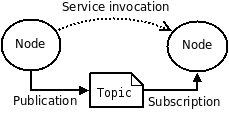
\includegraphics[width=\linewidth]{pictures/ROS_basic_concepts.png}
	\caption{Kommunikation zwischen Nodes}
\end{figure}

Die ROS-Software ist in sogenannten Nodes organisiert, welche die eigentlichen Berechnungen durchführen. Der ROS-Master hilft den Nodes sich zu finden und eine Verbindung aufzubauen. Die Kommunikation zwischen den Nodes erfolgt dann direkt untereinander über ein ROS spezifisches Protokoll dass auf TCP/IP aufsetzt. Nodes k\"onnen auf Topics ver\"offentlichen und diese abonnieren. \cite{rosConcepts}

Durch die Nodes k\"onnen Funktionalit\"aten wie Plannung, Pfadverfolgung, Sensorik, etc getrennt werden. Au{\ss}erdem k\"onnen so einfach Nodes von anderen Leuten genutzt werden. Dies erm\"oglicht es in kurzer Zeit eine Plattform zum Testen der Algorithmen aufzubauen, und ohne gro{\ss}en Aufwand Algorithmen durch Nodes zu implementieren. ROS-Nodes k\"onnen in C++ oder Python geschrieben werden. 
 

\section{Lokalisation}
\subsection{Odometrie}
{Die Odometrie beruht auf einer relativen Positionsbestimmung, dabei wird aus der vorher bekannten Position und der zur\"uckgelegten Weg-strecke die neue Position berechnet. Auf kurzen Distanzen liefert die Odometrie sehr genaue Ergebnisse. Mit wachsender Entfernung nehmen auch Fehler durch unterschiedliche Dr\"ucke in den Reifen oder eine verst\"arkte Reibung auf anderem Gel\"ande zu. Weitere Fehlerquelle sind h\"oheren Geschwindigkeiten und engeren Kurven, dort neigen die R\"ader zum Durchdrehen und Wegrutschen. Um das zu zeigen wird der Roboter \"ahnliche Pfade in langsamer und schneller Geschwindigkeit abfahren. 
	(Verkrüppeltes Bild einfügen)
	
	}
\subsection{Adaptive  Monte Carlo Localisation \cite{mclWiki}}
Im folgenden als AMCL abgek\"urzt, ist ein Algorithmus der mit Hilfe eines Partikelfilters die Position eines Roboters bestimmt. Dazu wird eine Karte der Umgebung ben\"otigt. Da die Pose zu Beginn nicht bekannt ist, stellt der Roboter Hypothesen \"uber auf der Karte an. Durch Laserscans, die durch die Bewegung des Roboters erfasst werden, vergleicht der Roboter die Messpunkte mit der Karte und bestimmt so seine Startpose. Die anf\"angliche Verteilung dieser Hypothesen auf der Karte kann verschieden sein. 
Bei uns ist sie Gau{\ss}-verteilt um gegebene anfängliche Pose. 

\begin{figure}[h]
	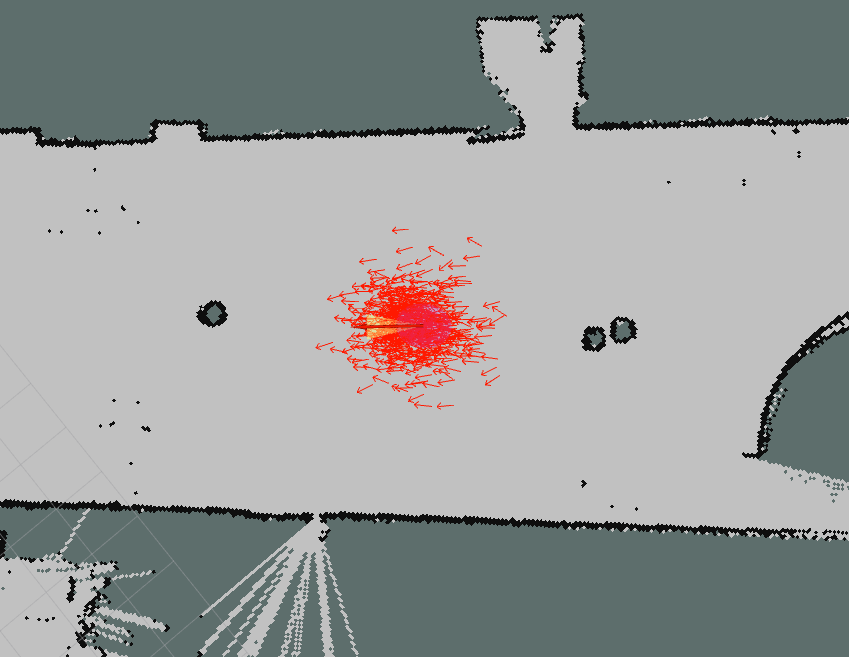
\includegraphics[width=\linewidth]{pictures/initial_distribution.jpg}
	\caption{Partikelverteilung in Anfangspose}
\end{figure}

Die Hypothesen kann man sich als virtuelle Roboter auf der Karte vorstellen. F\"ahrt der reale Roboter, so fahren auch die virtuellen Roboter, mit den gleichen Steuerungsbefehlen. Die realen Sensorwerte werden mit denen der virtuellen Robotern verglichen. Die virtuellen Roboter gewinnen ihre Sensormesswerte durch die Karte.

Je unstimmiger die Daten des virtuellen Roboters sind, desto unwahrscheinlicher ist die Hypothese dass der reale sich dort befindet. 

Probleme oder eine l\"angere Lokalisierungsdauer treten auf, wenn eine Umgebung keine markanten Anhangspunkte liefert, ein kreisf\"ormiger Raum mit glatten W\"anden zum Beispiel.

Unwahrscheinlichere Hypothesen werden gel\"oscht und neue im Bereich der wahrscheinlicheren aufgestellt, bzw. dort neue virtuelle Roboter erzeugt. Durch das L\"oschen der unwahrscheinlichen Posen, ist AMCL oft als Partikelfilter bezeichnet.





\begin{figure}[h]
	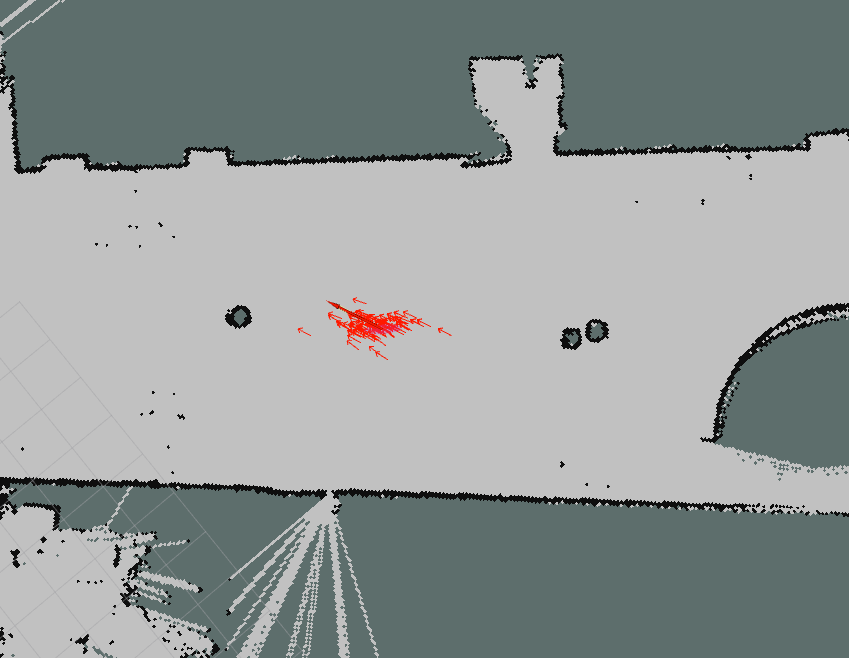
\includegraphics[width=\linewidth]{pictures/drive_little.jpg}
	\caption{Partikelverteilung nach kurzer Neuorientrierung durch Bewegung}
\end{figure}
 
Der virtuelle Roboter  mit besten den \"Ubereinstimmungen, ist die beste Estimation der Pose.
Je n\"aher die wahrscheinliche Hypothesen bei einander liegen, desto sicherer ist der Roboter sich seiner Pose. Dann kann die Anzahl der Hypothesen reduziert werden, daher dass A wie Adaptive aus AMCL. Dies reduziert die CPU Auslastung und den Speicher

Partikel und Gewicht, virtuelle Roboter nur in einem Satz erwähnen.

 


\subsection{Odometrie und AMCL im Vergleich}
Um die Lokalisation durch AMCL und Odometrie miteinander zu vergleichen f\"ahrt der Roboter einen "Acht"-f\"ormigen Pfad ab. Die Steuerung erfolgt manuell \"uber eine Joystick und wird zweimal in verschiedenen Geschwindigkeiten durchgef\"uhrt. Ein Problem entsteht am Anfang, da AMCL nur korrekt arbeitet, wenn die Startpose vorher durch den Benutzer auf den Punkt genau gesch\"atzt wird oder durch Bewegung des Roboters spezifiziert wird. Durch die Bewegung verliert aber die Odometrie an Genauigkeit und startet nicht mehr im Ursprung (0/0). Um Genauigkeit zu garantieren, wird ein Algorithmus verwendet, der die Koordinatensysteme nach der Kalibrierung transformiert.

\begin{figure}[h]
	\centering
	\subcaptionbox{Mit einer Geschwindigkeit $\leq$ 2km/h}{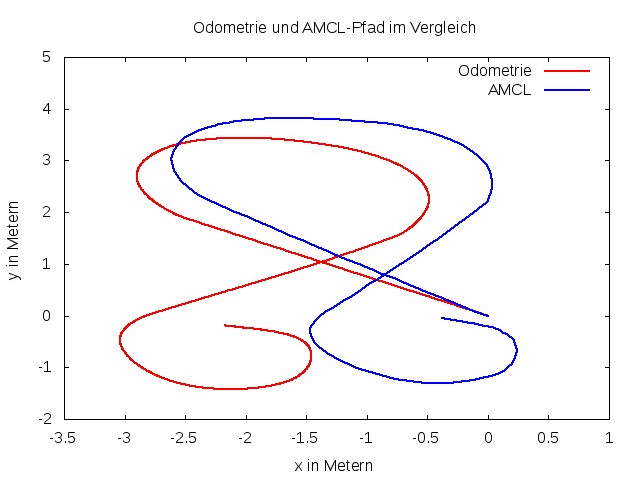
\includegraphics[width=\linewidth]{pictures/odo_amcl_comparision_slow.jpg}}\par\medskip
	\caption{ Odometrie und AMCL im Vergleich. }
\end{figure}




Man erkennt folgende Unterschiede ...

Im Experiment startet der Roboter im Ursprung und bereits zu Beginn kennzeichnet sich ab, dass der Odometriepfad fehlerhaft ist. Bis der Roboter wieder an der Startpose ist, summieren sich die Fehler auf und die Zielpose weicht bis zu 2 m von der Sartpose ab. Der AMCL Pfad dagegen, kehrt bis auf wenige Zentimeter zur Startpose zur\"uck. Zus\"atzlich muss in diesem Versuch die menschliche Ungenauigkeit, wie ungenaues Augenma{\ss}, beachtet werden. Aus dem Vergleich ist ersichtlich, dass der Fehler bei AMCL auch in der Distanz, also bei langen Pfaden, nicht gr\"o{\ss}er ist, w\"ahrend bei der Odometrie bei langer Laufzeit die Qualit\"at stetig abnimmt.


Nachteil AMCL: benötigt Karte, Pfad kann nicht in unbekannter Umgebung abgefahren werden

Vorteil: Odometrie ist h\"aufiger und schneller verf\"ugbar da der Rechenaufwand geringer ist. 


\section{Kartierung mit Gmapping} \cite{gmapping}
Die Lokalisation eines Roboters ben\"otigt eine Karte. Eine unbekannte Umgebung wird aus den Daten eines Laserscanners und den aktuellen Posedaten erfasst und von dem Algorithmus GMapping verarbeitet. Die Posedaten publiziert die Odometrie an das ROS Paket gmapping.
Die Herausforderung liegt dabei in der gleichzeitigen Lokalisierung und Kartierung, dem \textit{simultaneous localization and mapping} Problem kurz SLAM. Denn beide bedingen sich gegenseitig. Um zum Beispiel zwei Laserscans zu einer Karte zusammenzuf\"ugen, m\"ussen die relativen Posen der Aufnahmen bekannt sein. Also ein Lokalisierungsproblem. Und um sich mit dem Laserscanner zu lokalisieren, ben\"otigt man wiederum Kartendaten. \\

Die Idee des  \textit{Grid}Mappings ist, die Umgebung auf der Karte in bin\"aren Zufallsvariablen darzustellen. Die Variablen stellen Objekte in der Umgebung dar. Die Algorithmen, wie AMCL, werten die Zufallsvariablen aus. 


\begin{figure}[h]
	\centering
	\subcaptionbox{fehlerhafte Karte}{
		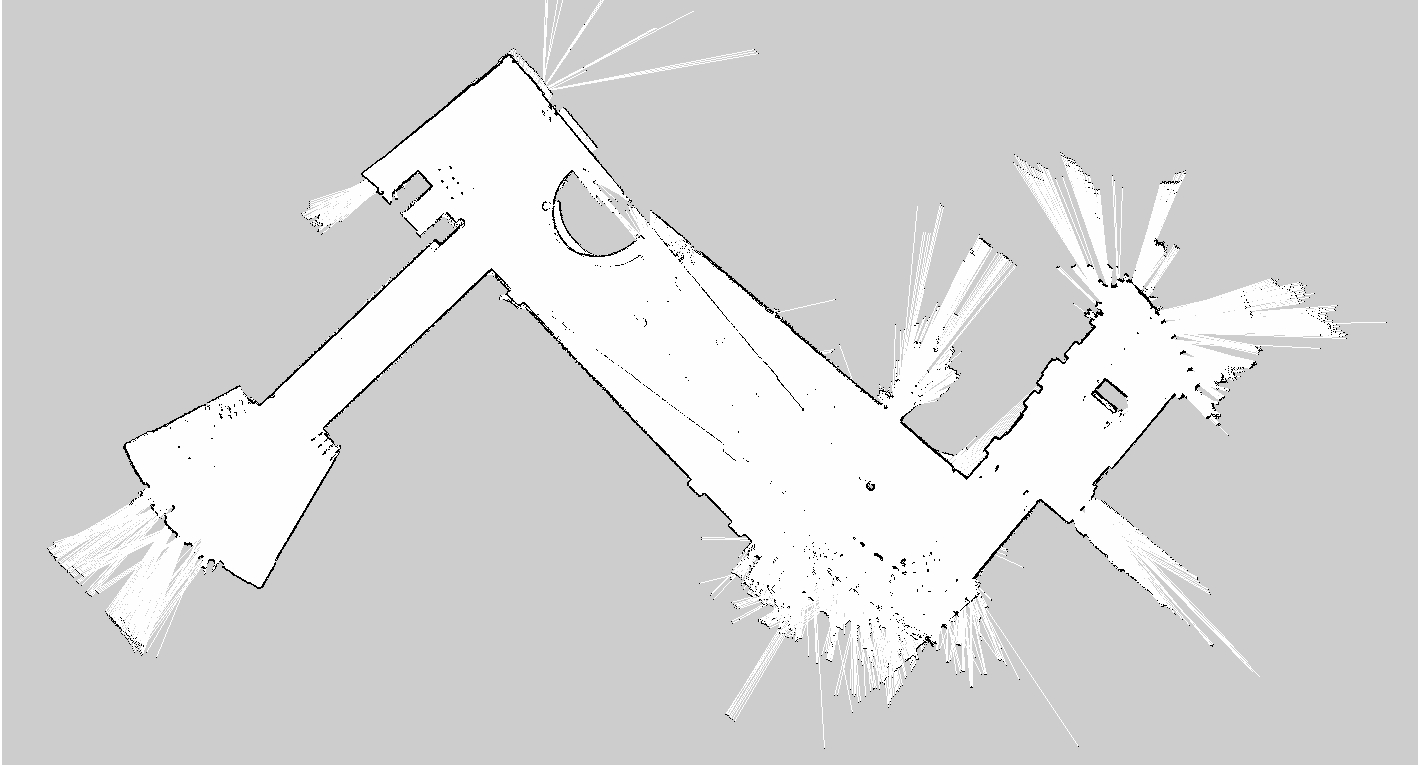
\includegraphics[width=0.45\textwidth]{pictures/firstMap.jpeg}}
	\subcaptionbox{korrekte Karte}{
		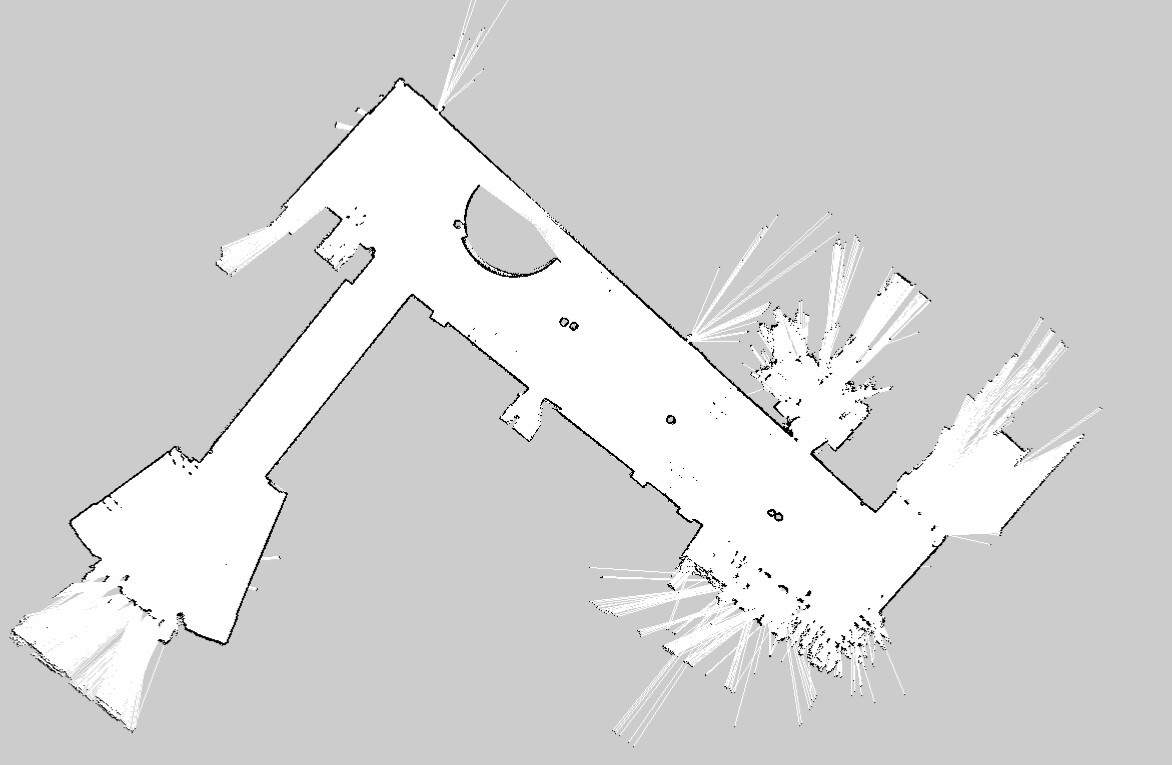
\includegraphics[width=0.45\textwidth]{pictures/correctMap.JPG}}
	\caption{Karten aufgezeichnet mit Gmapping}
\end{figure}


Das Untergeschoss des Informatikinstituts W\"urzburg ist mit einem Frauenhofer-Roboter, der mit einem Sick-Laserscanner ausgestattet ist, in einer 2D-Karte kartiert.  Um diese Karte korrekt aufzunehmen, werden nur so und soviel Partikel ben\"otigt. Die Aufnahme ist bis auf einen 1 cm genau und zeigt keine signifikanten Fehler. Bewegte Objekte wie Menschen werden erkannt und nicht in der Karte verzeichnet. Dagegen sorgt helles Licht, das durch die Fensterfronten scheint f\"ur eine Ungenauigkeit und kann nicht als klare Begrenzung festgestellt werden. F\"ur klare Linie wie W\"ande ist es wichtig, das Gel\"ande mit einem Geschwindgkeitslimit von 1 m/s abzufahren. 



Deutliche Unterschiede sind in den Karten von Figure 4 zu erkennen. Bild (a) zeigt eine Karte, die im ersten Versuch aufgenommen ist und aus Unwissenheit mit zu hoher Geschwindigkeit und nicht oft genug abgefahren ist. Im Vergleich dazu ist die Karte (b) durch langsameres und stetigeres Abfahren detailgetreuer und hat klare Linien.


eigene Karte einfügen. AMCL erwähnen.


\section{Pfadverfolgung}
\subsection{Pfadverfolgung mit Giovanni Indiveri}
\cite{Giovanni}


\begin{figure}[h]
	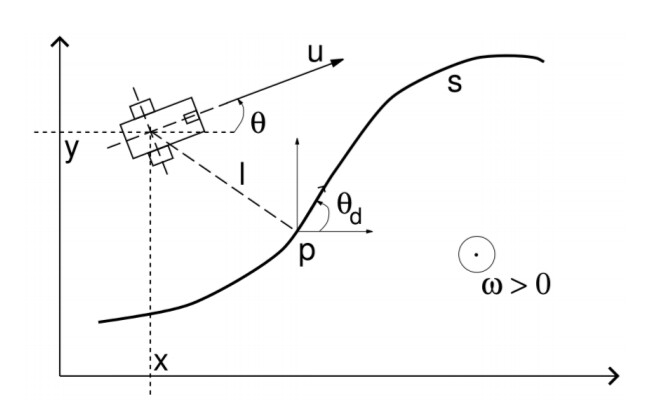
\includegraphics[width=\linewidth]{pictures/Pfadverfolgung.JPG}
	\caption{Modell der Pfadverfolgung}
\end{figure}

Der nicht-lineare Regler des Giovanni Indiveri und der Maria L. Corradini wird zur Pfadverfolgung verwendet. Die Implementierung garantiert nach Lyapunov, f\"ur einen beschr\"ankten, nicht-linearen Pfad, asymptotische Konvergenz und asymptotisch stabile Fehlerdynamik. Dabei muss sowohl die maximale Geschwindigkeit, als auch der minimale Wendekreis des Roboters beachtet werden. Schrittweise neue Berechnungen der Reglerparameter f\"uhren zu einer schnelleren Konvergenz. Hierzu verwendet der Algorithmus eine orthogonale Projektion auf den Roboter selbst. Das Modell in Figure 5 stellt den abzufahrenden Pfad dar. Der Pfad wird zur Vereinfachungen in lineare Teilschnitte gen\"ahert, wodurch sich die Gleichungen vereinfachen. Die Formel f\"ur die Winkelgeschwindigkeit $\omega$


\begin{equation}
 \omega=  \frac{u \kappa(s) cos(\tilde{\theta})}{1-l \kappa(s)}-h u l  \frac{sin(\tilde{\theta})}{\tilde{\theta}}-\gamma\tilde{\theta} :h\gamma > 0
\end{equation}\\

vereinfacht sich im linearen Fall $\kappa(s)=0$ zu \\

\begin{equation}
\omega= -h u y  \frac{sin(\theta)}{\theta}-\gamma\theta :h\gamma > 0
\end{equation}\\



Durch Koordinatentransformation, dient die x-Achse als die Fahrtrichtung des Robotors  und y (der Roboter-Pfad-Abstand) \"ubernimmt die Rolle des l. Der Winkel Theta wird durch das \"ubereinanderlegen zu null.




\subsection{Test und Implementierung von \texttt{gio\_path} auf einem realen Roboter}
Zun\"achst wird die Pfadverfolgung simuliert. Der Robotersimulator wird in ROS-Nodes organisiert und soll vorgebene Pfaddateien abfahren.
\\
\\
Um den \texttt{gio\_path} Algorithmus auf einem realen Roboter zu testen, wird eine ROS-Node verwendet. Diese benutzt  \texttt{gio\_path} um einen realen Roboter zu steuern.
\\

  \textbf{bool} pathDone\\
  controller setPath( super path ) \\
  \textbf{while}(!pathDone)                  \\
	  controller setPose(currentPose)\\
	  pathDone = controller getNextState(wheelcontrol) \\
	  publish(wheelCOntrol)
\\

\begin{figure}[h]
	\centering
	\subcaptionbox{niedrige Geschwindigkeit}{
		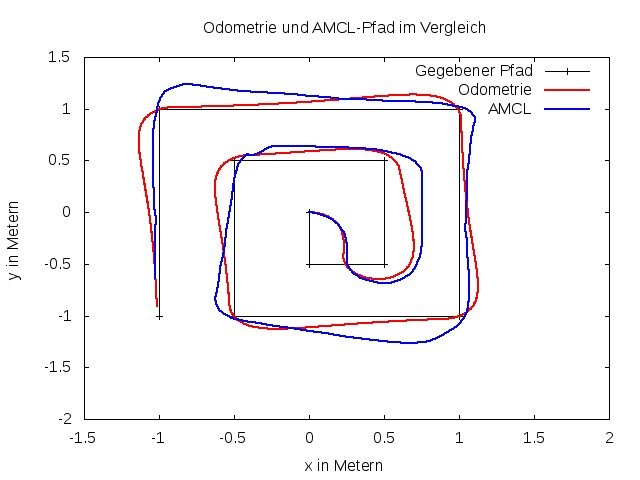
\includegraphics[width=0.45\textwidth]{pictures/path_odometry_slow.jpg}}
	\subcaptionbox{erh\"ohte Geschwindigkeit}{
		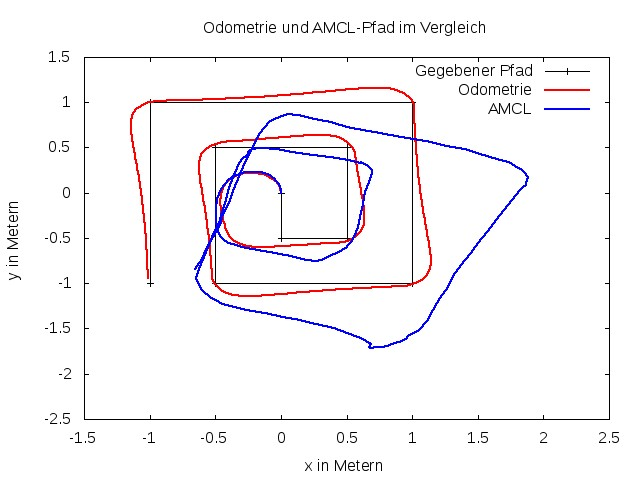
\includegraphics[width=0.45\textwidth]{pictures/path_odometry_fast.jpg}}
	\caption{Pfadverfolgung}
\end{figure}

Die Autoren entscheiden sich als Testpfad eine Spirale zu nutzen. Die Datei enth\"alt Punkte in spiralf\"ormiger, eckiger Anordnung. In dem Vergleich wird der Pfad zweimal abgefahren, einmal in niedriger und einmal hoher Geschwindigkeit. Zu Beobachten ist, dass AMCL bei geringer Geschwindigkeit exakt arbeitet und die Punkte nur auf wenige Zentimeter verfehlt. Bei erh\"oter Geschwindigkeit ist eine Spirale nicht mehr zu erkennen. Die Odometrie zeichnet in beiden F\"allen eine korrekte Spirale auf. Der Grund ist, dass Odometrie unabh\"angig der Umgebung, also ohne Karte, arbeitet und trotz optisch fehlerhaften Pfad die Punkte korrekt skizziert.


\section{Zusammenfassung und Ausblick}

Es zeigt sich das Odometrie schlechter als AMCL ist.

\newpage
{%\small                   % use small if you need it
	\bibliographystyle{plain}
	\bibliography{paper.bib}       % use a bib-file paper.bib to collect

\end{document}



